\section{City Bike Dataset}
For this project, our main dataset is the \href{https://www.citibikenyc.com/system-data}{\underline{Citi Bike system dataset}}, a publicly available dataset tracking trips made through New York City's Citi Bike share network since 2013.

\subsection{Dataset Structure}
Released monthly as CSV files, these records log every completed ride, with high-volume months split across multiple files.
Each row represents a single trip, offering detailed attributes that characterize the journey.

\subsubsection{Original Structure}
The original dataset includes the following columns:
\begin{itemize}
    \item \textbf{Ride ID}: A unique identifier for each bike trip.
    \item \textbf{Rideable Type}: The type of bike used for the trip (``classic'' or ``electric'').
    \item \textbf{Started At}: A timestamp indicating when the trip started.
    \item \textbf{Ended At}: A timestamp indicating when the trip ended.
    \item \textbf{Start Info}: Information about the station and location where the trip started, structured as:
          \begin{itemize}
              \item \textbf{Station Name}: The name of the starting station.
              \item \textbf{Station ID}: The identifier of the starting station.
              \item \textbf{Latitude}: The latitude coordinate of the starting station.
              \item \textbf{Longitude}: The longitude coordinate of the starting station.
          \end{itemize}
    \item \textbf{End Info}: Information about the destination station, structured equally to Start Info.
    \item \textbf{User Type}: The type of user (``member'' or ``casual'').
\end{itemize}

\subsubsection{Extracted Features}
Additional per-trip features were derived to support the analysis:
\begin{itemize}
    \item \textbf{Trip Duration}: The duration of the trip in seconds, calculated as $\text{Ended At} - \text{Started At}$.
    \item \textbf{Trip Distance}: The straight-line distance between the start and end stations, computed using the Haversine formula and scaled by a circuity factor of $1.3$ to approximate actual street routes.
\end{itemize}

Then, these individual trips were aggregated to derive:
\begin{itemize} 
    \item \textbf{Station Activity}: The total number of trips starting and ending at each station during a given time period, calculated by grouping trips by station.
    \item \textbf{Origin-Destination Flow}: The total number of trips made between each pair of stations within a given time period, calculated by grouping trips by station pair.
\end{itemize}

\subsection{Analysis and Insights}
For transparency and reproducibility, the complete workflow is available in our \href{https://github.com/davide-dona/nyc-bike-data-visualization/blob/main/src/notebooks/analysis.ipynb}{\underline{Jupyter notebook}}.
Using the February 2025 trip dataset, the following sections examine temporal, spatial, and behavioral usage patterns.
Rather than offering a comprehensive study of the Citi Bike system, this prior analysis serves to justify our visualization design choices.

\paragraph{Temporal Analysis}
Figure~\ref{fig:rides_time} illustrates distinct variations in demand across different hours and days of the week.
Weekday trips peak during standard commuting hours, whereas weekend usage shifts toward smooth patterns.
These temporal patterns provide a foundation for designing visualizations that highlight the system's daily, weekly, and hourly usage trends, enabling users to explore how demand fluctuates over time.

\begin{figure}[ptb]
    \centering
    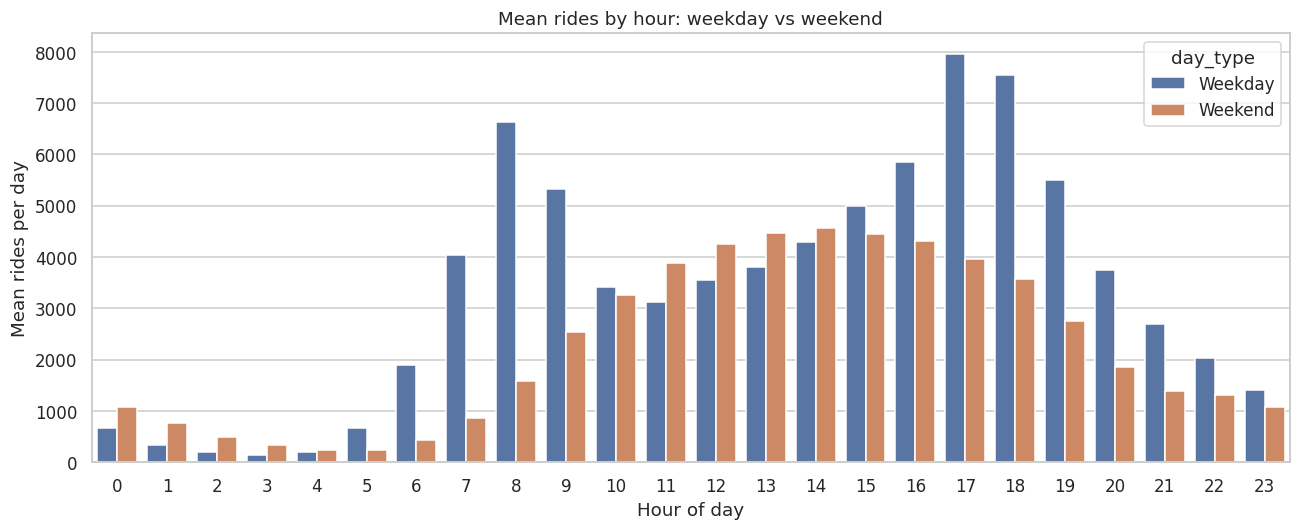
\includegraphics[width=\textwidth]{../media/technical/rides_time.png}
    \caption{Distribution of trips by hour of the day and weekday/weekend.}
    \label{fig:rides_time}
\end{figure}

\paragraph{Spatial Analysis}
Figure~\ref{fig:rides_stations} highlights the distribution of station origins across the city.
Station popularity and trip flows reveal that demand is concentrated around Manhattan and other high-density areas, with some stations acting as important origins.
Ultimately, it's possible to see that the dataset's spatial distribution is able to cover the entire city, providing a comprehensive view of the Citi Bike system's reach and usage patterns.

\begin{figure}[ptb]
    \centering
    
\includegraphics[width=0.5\textwidth]{../media/technical/rides_stations.png}
    \caption{Distribution of trips by station of origin, aggregated into $300$ m cells so that every colour class maps to an exact number of trips.}
    \label{fig:rides_stations}
\end{figure}

\paragraph{User/Bike Type Behaviour Analysis}
As shown in Figure~\ref{fig:rides_type}, both casual riders and members prefer electric bikes.
Because e-bikes allow users to cover greater distances faster, overall trip durations tend to be shorter. 
However, casual riders still take longer trips than members across both bike types, whereas members maintain consistently short ride times regardless of vehicle choice.
These contrasting behaviors highlight distinct usage patterns, useful to inform in the design of visualizations.
\begin{figure}[ptb]
    \centering
    
\includegraphics[width=0.8\textwidth]{../media/technical/rides_type.png}
    \caption{Distribution of trips by user/ride type based on rides and trip length.}
    \label{fig:rides_type}
\end{figure}

\paragraph{Trip Duration and Distance}
Figures~\ref{fig:rides_duration} and~\ref{fig:rides_distance} provide additional insight into mobility behaviour.
Most trips are relatively short, while longer rides are less frequent and often correspond to recreational usage.
It's important to note that durations begin at one minute, as Citi Bike removes trips shorter than 60 seconds at the source.
This, together with other outliers, are compacted into the final or initial bins of the histograms.

\begin{figure}[ptb]
    \centering
    \begin{minipage}[t]{0.45\textwidth}
        \centering
        
\includegraphics[width=\textwidth]{../media/technical/rides_duration.png}
        \caption{Distribution of trip durations.}
        \label{fig:rides_duration}
    \end{minipage}
    \hfill
    \begin{minipage}[t]{0.45\textwidth}
        \centering
        
\includegraphics[width=\textwidth]{../media/technical/rides_distance.png}
        \caption{Distribution of trip straight-line distances.}
        \label{fig:rides_distance}
    \end{minipage}
\end{figure}

\subsection{Data Quality}
To prevent misleading visual representations and maintain data integrity, we identified several data quality issues in the raw Citi Bike dataset.

\paragraph{Different Legacy Structure}
In 2020, Citi Bike updated its trip data schema, introducing column and formatting changes that differ from the 2013--2019 legacy format (detailed in our \href{https://github.com/davide-dona/nyc-bike-data-visualization/blob/main/src/notebooks/analysis.ipynb}{\underline{analysis notebook}}).
Despite these structural discrepancies, the historical data remains still valuable, justifying the need for reformatting them.

\paragraph{Missing Station Values}
A tiny fraction of trips contain missing values, confined entirely to station-related fields.
The issue predominantly impacts end-of-trip attributes: in the representative month, roughly $4{,}800$ trips ($0.24\%$) lack an end station identifier, compared to just $0.03\%$ for start stations.
This gap likely stems from abandoned bikes or off-dock returns.

\paragraph{Trip Outliers}
Beyond missing values, a small number of trips are clear outliers.
In a representative month, about $315$ trips ($0.02\%$) last up to $25$ hours, appearing in the final bin of the duration histogram (Figure~\ref{fig:rides_duration}).
These likely reflect unreturned bikes rather than continuous rides.
Additionally, around $27{,}000$ trips ($1.4\%$) start and end at the same station, resulting in a zero straight-line distance (Figure~\ref{fig:rides_distance}).
Finally, some trips report impossible distances ($11{,}000$~km as an example), due to corrupted station coordinates.

\paragraph{Biases}
This dataset carries certain inherent limitations.
Because it relies exclusively on the Citi Bike system dataset, the findings may not accurately reflect the demographics of the entire population of cyclists in New York City.
Additionally, trip distances are calculated using the Haversine formula between the start and end stations; this straight-line metric serves only as a geometric approximation and cannot account for the actual routes or detours taken by riders.
